% !TEX program = pdflatex
%
% Semantic identification of congestion regions in São Paulo public transport
% using the Olho Vivo API and CB-SMoT.
%
% Build: pdflatex main && bibtex main && pdflatex main && pdflatex main
%
\documentclass[11pt,a4paper]{article}

\usepackage[utf8]{inputenc}
\usepackage[T1]{fontenc}
\usepackage[english]{babel}
\usepackage{lmodern}
\usepackage{microtype}
\usepackage{geometry}
\geometry{margin=2.5cm}

\usepackage{graphicx}
\usepackage{booktabs}
\usepackage{amsmath}
\usepackage{amssymb}
\usepackage{algorithm}
\usepackage{algpseudocode}
\usepackage{hyperref}
\usepackage{url}
\usepackage{subcaption}

\graphicspath{{figures/}}

\hypersetup{
    colorlinks=true,
    linkcolor=black,
    citecolor=blue,
    urlcolor=blue
}

\title{Semantic Identification of Congestion Regions in\\
       São Paulo Public Transport using the Olho Vivo API}

\author{Marcos Filipe Lino}

\date{}

\begin{document}
\maketitle

\begin{abstract}
Public transport fleets in large metropolitan areas spend a substantial
share of their operating time in low-speed conditions caused by
congestion, signalized intersections, and passenger-service stops. We
apply CB-SMoT (Clustering-Based Stops and Moves of Trajectories) to
vehicle-position data published by the São Paulo Transport Authority
(SPTrans) through the \emph{Olho Vivo} REST API, in order to
semantically label recurring low-speed regions as candidate congestion
hotspots. A case study on bus line 8003-10, which links Terminal Lapa to
Avenida dos Remédios, is conducted over a trajectory dataset of
$2{,}580$ GPS fixes. Running CB-SMoT with several combinations of
minimum-time and maximum-average-speed parameters and then clustering
the resulting segments spatially, we identify twelve
recurrent stop regions. Manual inspection of street-level imagery
confirms that the recovered regions correspond to viaducts, signalized
intersections, and heavily trafficked corridors. Scheduled bus stops are
not, in general, among the recovered regions, suggesting that boarding
dwell times do not dominate the low-speed behavior observed on the
route.
\end{abstract}

\section{Introduction}
\label{sec:introduction}

São Paulo operates one of the largest urban bus networks in the Americas
and makes its live vehicle-position feed available to the public through
the \emph{Olho Vivo} REST API. While the data is rich, each record
arrives as an unlabeled $(x,y,t)$ triple: the same point can represent
free-flow motion, waiting at a red light, boarding passengers, or being
stuck in traffic.

Stop-and-move segmentation is a long-standing problem in trajectory
mining~\cite{alvares2007}. Among the clustering-based approaches,
CB-SMoT~\cite{palma2008} is attractive because it operates on a single
trajectory, requires only two interpretable parameters (a maximum
average speed and a minimum duration), and returns geometrically
meaningful segments that can later be enriched with external semantic
layers.

This paper asks: \emph{can CB-SMoT, applied to Olho Vivo data, recover
recurrent low-speed regions that correspond to congestion hotspots on
São Paulo bus routes?} Our contributions are:
\begin{enumerate}
    \item A concrete CB-SMoT pipeline for SPTrans data: ingesting live
    vehicle positions, persisting trajectories, running the
    segmentation algorithm, and aggregating detected segments into
    recurrent regions.
    \item A case study on line 8003-10 (Terminal Lapa $\leftrightarrow$
    Avenida dos Remédios) covering $2{,}580$ trajectory points, in
    which twelve recurrent low-speed regions are identified and
    validated against street-level imagery.
    \item Evidence that scheduled bus stops are \emph{not} the dominant
    cause of low-speed events on this route; the recovered hotspots
    coincide instead with viaducts, avenue bottlenecks, and signalized
    intersections.
\end{enumerate}

Section~\ref{sec:concepts} reviews the trajectory-mining concepts we
build on. Section~\ref{sec:method} describes the CB-SMoT algorithm as
implemented here. Section~\ref{sec:pipeline} presents the data
pipeline. Section~\ref{sec:experiment} reports the case study and
results. Section~\ref{sec:discussion} discusses limitations and
Section~\ref{sec:conclusion} concludes.

\section{Background}
\label{sec:concepts}

\paragraph{Trajectories of moving objects.}
A \emph{trajectory} is a time-ordered sequence of geographic positions
recorded for an object as it moves; a trajectory enables both the
tracking of the object and the later analysis and interpretation of its
movement~\cite{bogorny}. Figure~\ref{fig:trajectory_concept} illustrates
the concept together with a representative tabular layout.

\begin{figure}[t]
    \centering
    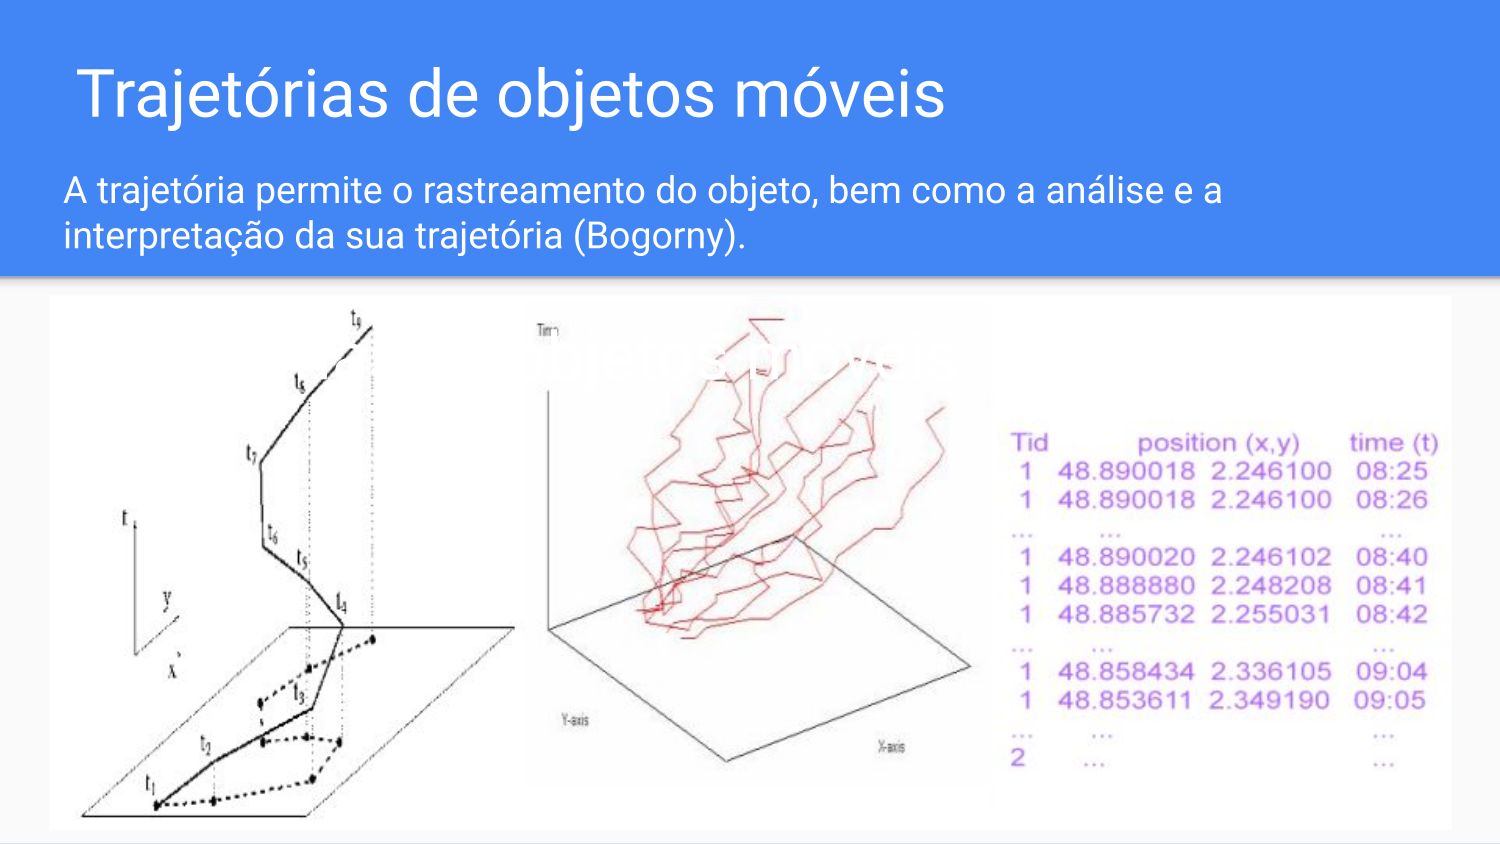
\includegraphics[width=0.85\linewidth]{slide-03.png}
    \caption{Trajectories of moving objects (adapted from the study
    presentation). Left: 3D time-enriched path; middle: 2D projection;
    right: tabular representation of the same data.}
    \label{fig:trajectory_concept}
\end{figure}

\paragraph{Trajectory data analysis.}
Raw-trajectory analysis seeks to extract behavioral patterns — such as
\emph{leadership}, \emph{flock}, \emph{encounter}, and
\emph{convergence} — from groups of trajectories, typically by
geometric reasoning over the $(x,y,t)$ traces~\cite{giannotti}.

\paragraph{Semantic trajectory analysis.}
A raw trajectory can be enriched with semantic labels chosen according
to the application context. Figure~\ref{fig:semantic_trajectory}
contrasts a raw trace (top) with two semantic enrichments: the same
trace interpreted as a tourism itinerary (middle) and as a mobility
pattern that exposes a \emph{Traffic Jam} and a \emph{Cross Road}
(bottom). The present work focuses on the second kind of enrichment:
identifying congestion regions within bus trajectories.

\begin{figure}[t]
    \centering
    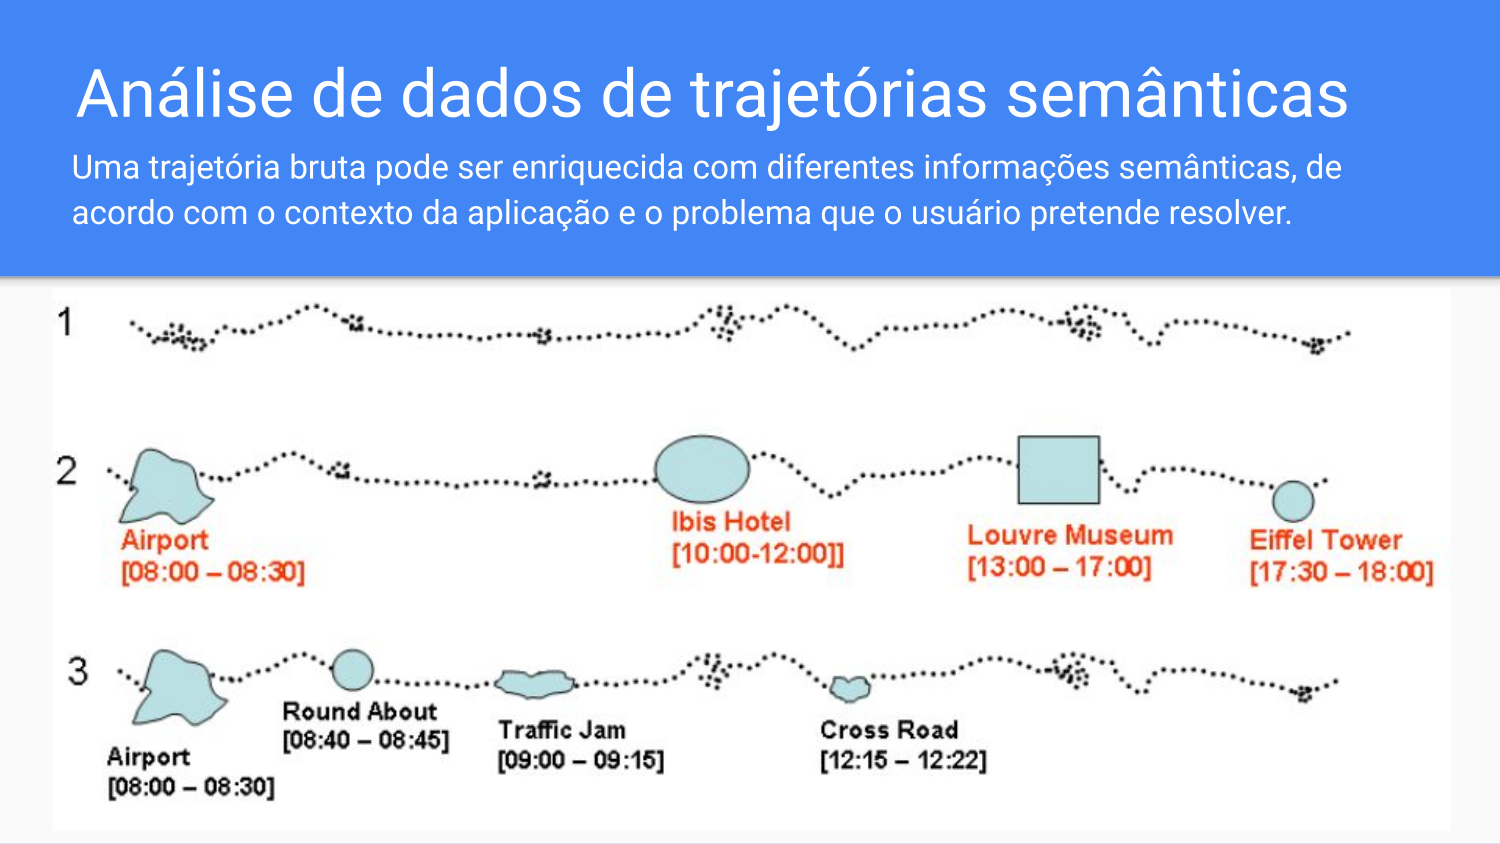
\includegraphics[width=0.85\linewidth]{slide-05.png}
    \caption{A raw trajectory (row 1) can be enriched with semantics
    chosen by the analyst (rows 2 and 3).}
    \label{fig:semantic_trajectory}
\end{figure}

\section{Method: CB-SMoT}
\label{sec:method}

Bogorny~\cite{bogorny} describes two families of algorithms for
instantiating the \emph{Stops and Moves} model: intersection-based
methods (SMoT), which rely on pre-defined points of interest, and
clustering-based methods (CB-SMoT), which derive stops directly from
the trajectory. Because the set of interesting regions is not known in
advance for congestion analysis, we adopt CB-SMoT.

\subsection{Problem setting}
Let $\mathcal{T} = \langle p_1, p_2, \ldots, p_n \rangle$ be a sequence
of GPS fixes for a single vehicle, sorted by time, with each $p_i$
carrying a timestamp $t_i$ and a longitude--latitude pair $(x_i, y_i)$.
Figure~\ref{fig:cbsmot_overview} shows the task: recover the
sub-sequences of $\mathcal{T}$ that correspond to congestion regions.

\begin{figure}[t]
    \centering
    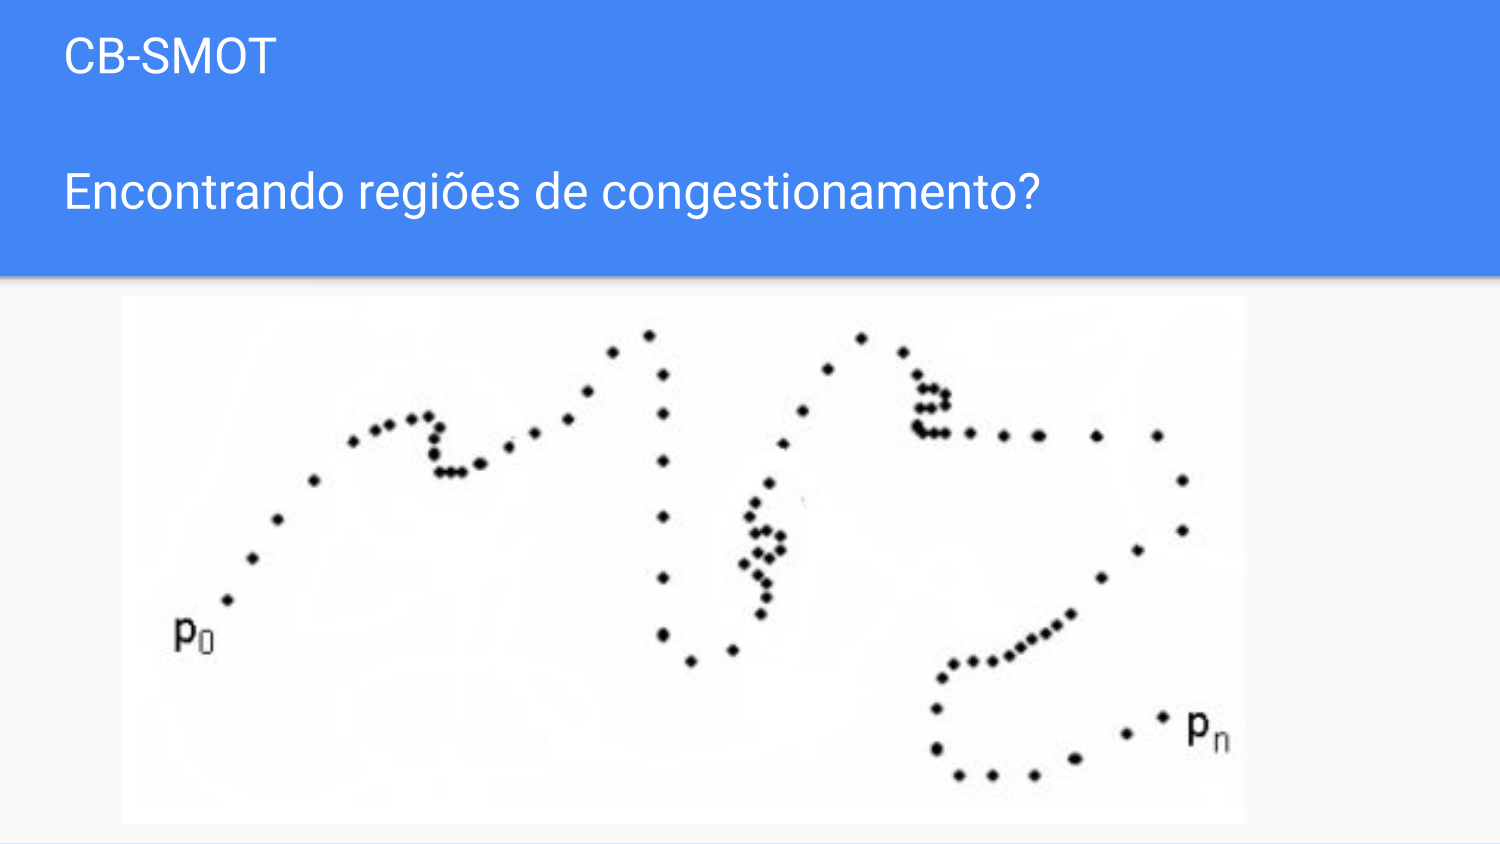
\includegraphics[width=0.75\linewidth]{slide-10.png}
    \caption{CB-SMoT input: a single trajectory of GPS fixes from
    $p_0$ to $p_n$. Visual inspection already suggests several regions
    where consecutive points cluster tightly; the algorithm recovers
    these regions automatically.}
    \label{fig:cbsmot_overview}
\end{figure}

\subsection{Point-wise distance and speed}
Between two consecutive fixes $p_{i-1}$ and $p_i$, the great-circle
distance in meters is given by
\begin{equation}
    d_{i} = R \cdot 2 \arcsin \sqrt{%
        \sin^{2}\!\left(\tfrac{\Delta \phi}{2}\right) +
        \cos\phi_{i-1}\cos\phi_i \sin^{2}\!\left(\tfrac{\Delta\lambda}{2}\right)
    },
\end{equation}
with $\phi$ the latitude, $\lambda$ the longitude, and
$R = 6{,}371 \times 10^{3}$~m. Let $\Delta t_i = t_i - t_{i-1}$ (in
seconds) and $v_i = d_i / \Delta t_i$ the pair-averaged speed. When the
feed repeats the same timestamp and coordinates on consecutive polls, we
treat that pair as a duplicate stationary observation: it contributes no
additional duration, but it also does not terminate an in-progress stop.

\subsection{Segmentation rule}
A stop $S$ is a maximal contiguous run of indices
$\{i, i+1, \ldots, j\}$ such that, for every consecutive pair inside
the run,
\begin{equation}
    \Delta t_k < \tau_{\text{gap}}
    \quad\text{and}\quad
    v_k < v_{\max},
    \qquad k = i+1, \ldots, j,
    \label{eq:stoprule}
\end{equation}
and whose total elapsed time exceeds $T_{\min}$:
\begin{equation}
    \sum_{k=i+1}^{j} \Delta t_k > T_{\min}.
    \label{eq:mintime}
\end{equation}
Figure~\ref{fig:cbsmot_variant} illustrates the rule graphically: the
average speed is plotted against time and the algorithm selects
contiguous intervals that (i) lie below the $v_{\max}$ threshold and
(ii) are longer than \textit{min-time}.

\begin{figure}[t]
    \centering
    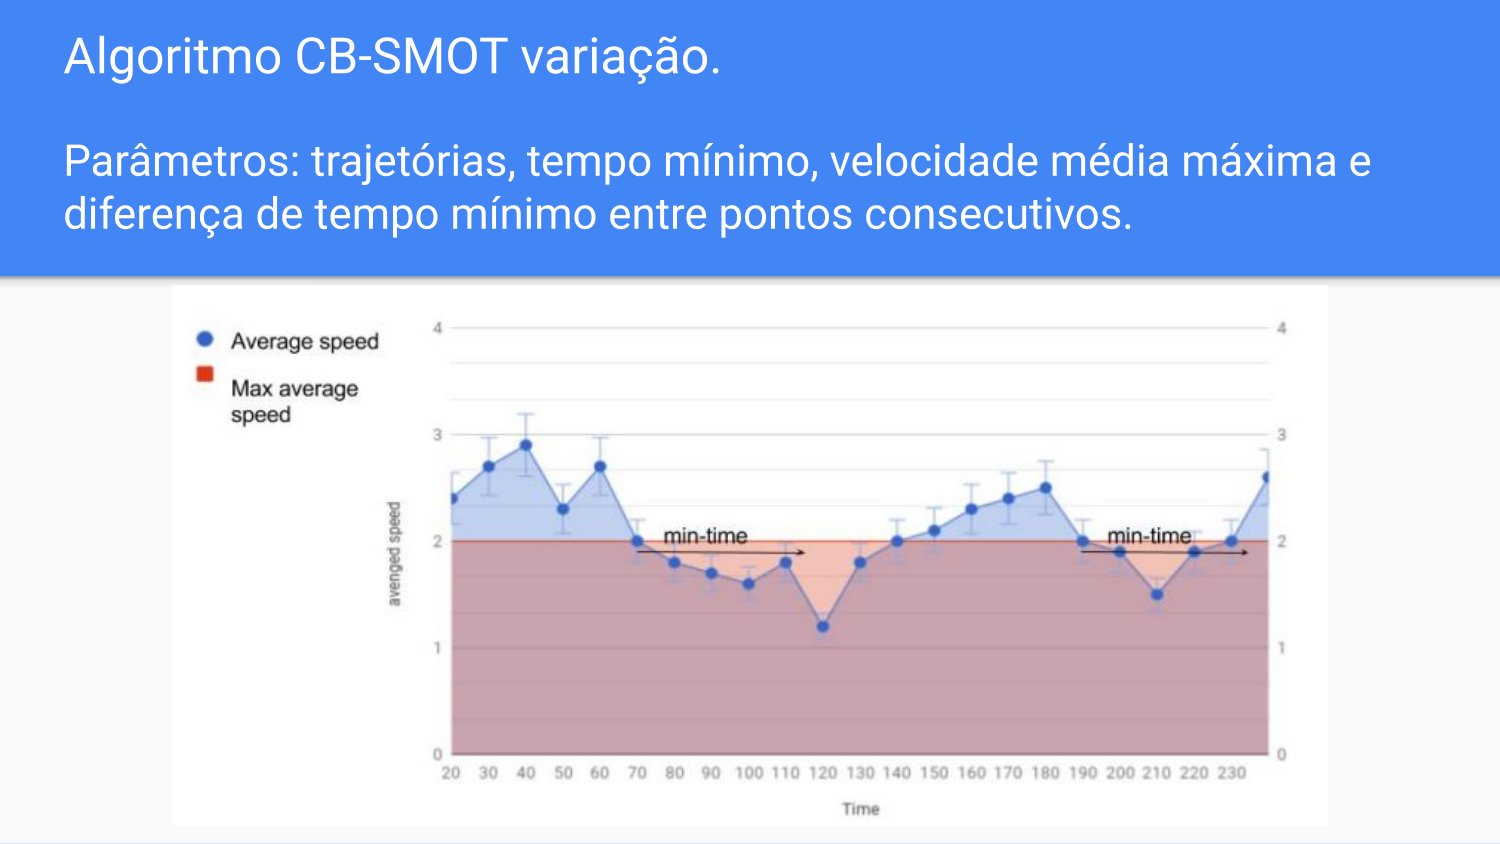
\includegraphics[width=0.8\linewidth]{slide-15.png}
    \caption{CB-SMoT decision rule on a speed--time plot. Two candidate
    stops are highlighted: both intervals lie below the maximum-average
    speed line and both exceed \textit{min-time}.}
    \label{fig:cbsmot_variant}
\end{figure}

The gap bound $\tau_{\text{gap}}$ prevents sparse data from
artificially inflating a segment: two fixes separated by more than
$\tau_{\text{gap}}$~s cannot belong to the same stop. In this work we
set $\tau_{\text{gap}} = 20$~s, matching the $\approx$15~s Olho Vivo
polling interval with a small tolerance.

Pseudocode is given in Algorithm~\ref{alg:cbsmot}.

\begin{algorithm}
\caption{CB-SMoT segmentation on a single trajectory.}
\label{alg:cbsmot}
\begin{algorithmic}[1]
\Require trajectory $\mathcal{T}$, parameters $v_{\max}, T_{\min}, \tau_{\text{gap}}$
\Ensure list of stops $\mathcal{S}$
\State $\mathcal{S} \gets \emptyset$;\; $S \gets \bot$;\; $p_{\text{prev}} \gets p_1$
\For{$i = 2$ \textbf{to} $n$}
    \State compute $\Delta t_i, d_i$
    \State set $v_i \gets d_i / \Delta t_i$ if $\Delta t_i > 0$; set $v_i \gets 0$ if $\Delta t_i = 0$ and $d_i = 0$; otherwise set $v_i \gets \infty$
    \If{$\Delta t_i < \tau_{\text{gap}}$ \textbf{and} $v_i < v_{\max}$}
        \If{$S = \bot$}
            \State $S \gets \text{new Stop}()$; add $p_{\text{prev}}$ to $S$ with distance $0$
        \EndIf
        \State add $p_i$ to $S$ with distance $d_i$
    \Else
        \If{$S \neq \bot$ and $\text{duration}(S) > T_{\min}$}
            \State append $S$ to $\mathcal{S}$
        \EndIf
        \State $S \gets \bot$
    \EndIf
    \State $p_{\text{prev}} \gets p_i$
\EndFor
\If{$S \neq \bot$ and $\text{duration}(S) > T_{\min}$}
    \State append $S$ to $\mathcal{S}$
\EndIf
\State \Return $\mathcal{S}$
\end{algorithmic}
\end{algorithm}

\section{Pipeline}
\label{sec:pipeline}

The implementation is a four-stage file-based pipeline:
\emph{ingest}, \emph{process}, \emph{regions}, and \emph{report}. Each
stage reads and writes columnar files; the core CB-SMoT segmentation in
Section~\ref{sec:method} is implemented in pure Python, and the
pipeline wraps it with thin modules built on \texttt{pandas},
\texttt{shapely}, and \texttt{scikit-learn}.

\paragraph{Ingest.}
A thin REST client authenticates once with the Olho Vivo API and then
polls \texttt{/Posicao/Linha} every 15~s for a configurable list of
\texttt{codigoLinha} values, extracting
\{\texttt{vehicle\_id}, \texttt{route\_id}, \texttt{datetime},
\texttt{latitude}, \texttt{longitude}\} per vehicle per tick. The
\texttt{datetime} field stores the observation time of the poll rather
than the raw \texttt{ta} value published by the API, because \texttt{ta}
can repeat while a bus remains stationary. The original \texttt{ta}
timestamp is preserved separately for provenance.

\paragraph{Process.}
Trajectories are grouped by \texttt{vehicle\_id}, sorted by time, and
passed to Algorithm~\ref{alg:cbsmot}. Each detected stop becomes one
segment row with the fields listed in Table~\ref{tab:schema}.

\paragraph{Regions.}
The segment output is then clustered into recurrent regions using DBSCAN
over segment centroids with a haversine distance metric. This is the
step that turns repeated per-vehicle low-speed episodes into route-level
hotspot candidates.

\paragraph{Report.}
Aggregate statistics — total segments, average duration and speed,
top-$N$ routes by segment count, and hour-of-day histogram — are
computed with standard group-by operations and printed to the console.

\begin{table}[t]
    \centering
    \caption{Detected-segment schema.}
    \label{tab:schema}
    \begin{tabular}{@{}lll@{}}
        \toprule
        Column & Type & Description \\
        \midrule
        \texttt{vehicle\_id} & integer & Bus prefix from SPTrans \\
        \texttt{route\_id} & integer & Line code (\texttt{codigoLinha}) \\
        \texttt{start\_time} & timestamp & First fix in the segment \\
        \texttt{end\_time} & timestamp & Last fix in the segment \\
        \texttt{duration\_seconds} & float & Elapsed time, Eq.~\eqref{eq:mintime} \\
        \texttt{distance\_meters} & float & Haversine path length \\
        \texttt{num\_points} & integer & GPS fixes forming the segment \\
        \texttt{average\_speed\_mps} & float & \texttt{distance / duration} \\
        \texttt{geometry\_wkt} & string & \texttt{LINESTRING} geometry (WGS84) \\
        \bottomrule
    \end{tabular}
\end{table}

\section{Case Study: Line 8003-10}
\label{sec:experiment}

\subsection{Setup}

The modified CB-SMoT algorithm was applied to line 8003-10, which links
\emph{Terminal Lapa} to \emph{Avenida dos Remédios}
(Figure~\ref{fig:route_map}). The trajectory dataset consists of
$2{,}580$ GPS fixes collected from the Olho Vivo API while buses were
active on the route.

\begin{figure}[t]
    \centering
    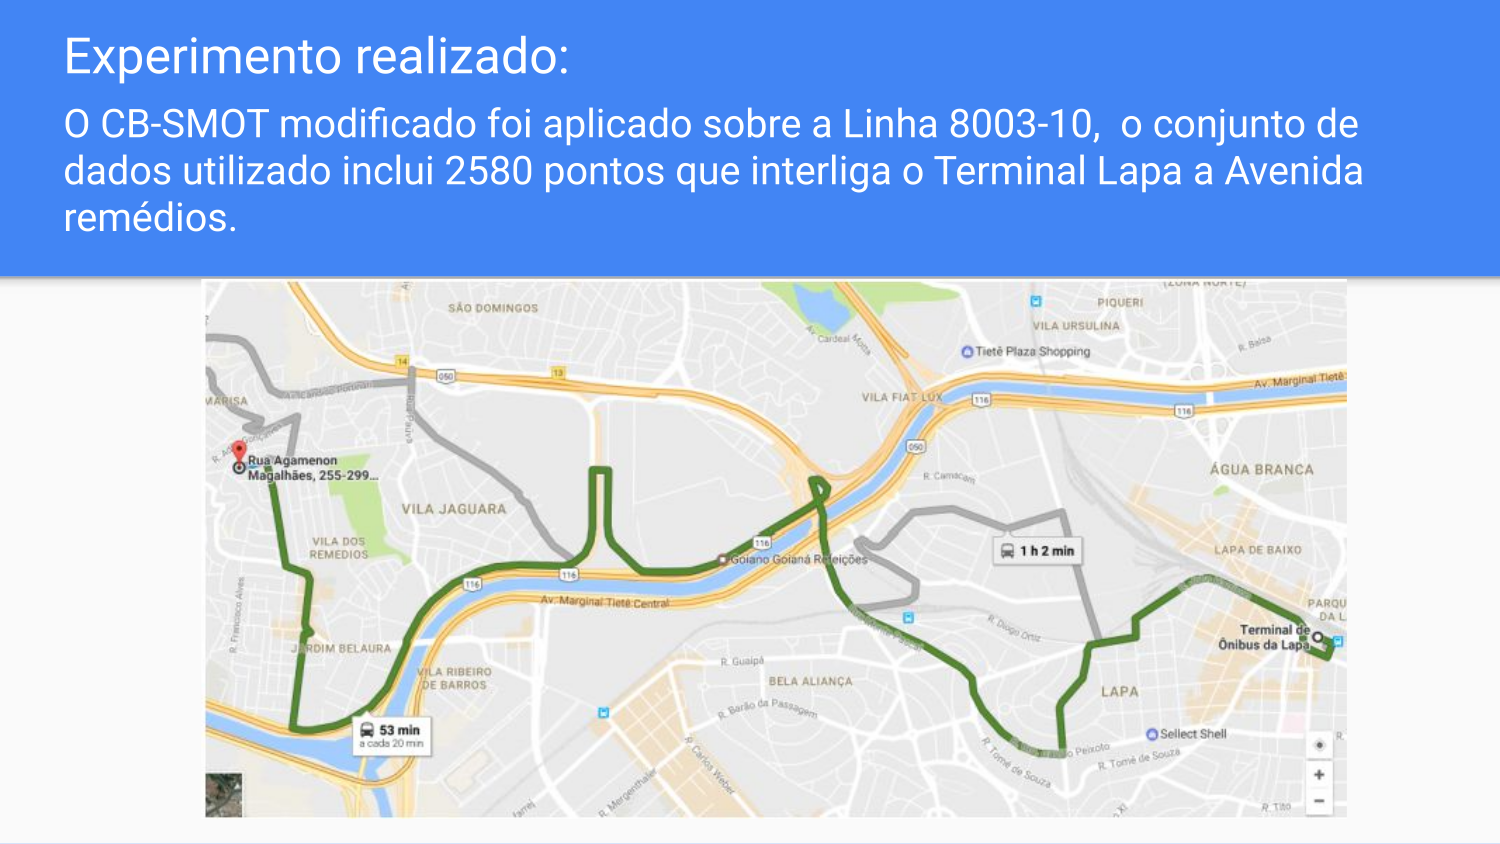
\includegraphics[width=0.85\linewidth]{slide-16.png}
    \caption{Line 8003-10: Terminal Lapa $\leftrightarrow$ Avenida dos
    Remédios. The route traverses the Marginal Tietê expressway, a
    known high-volume corridor.}
    \label{fig:route_map}
\end{figure}

\subsection{Parameter sweep}

The algorithm was run with several combinations of $T_{\min}$ and
$v_{\max}$. For each run, the detected segments were clustered into
recurrent regions. The goal was to identify the \emph{worst cases} —
i.e.\ regions where the low-speed behavior was sufficiently prolonged to
plausibly correspond to real congestion rather than to transient
slowdowns such as passenger boarding or a single signal cycle.

Table~\ref{tab:stops} lists the twelve stop regions recovered across
the sweep. Regions labeled with $v_{\max}=1$~m/s capture the most
severe slowdowns; the two regions labeled with $v_{\max}=2$~m/s reflect
a slightly looser definition of congestion. The street-address labels in
the table are descriptive annotations assigned after clustering by
manual map inspection; they are not geocoded automatically by the code.

\begin{table}[t]
    \centering
    \caption{Stop regions identified on line 8003-10. The $T_{\min}$
    column is in seconds.}
    \label{tab:stops}
    \begin{tabular}{@{}clcl@{}}
        \toprule
        id & $T_{\min}$ (s) & $v_{\max}$ (m/s) & Location \\
        \midrule
        1  & 1140 & 1 & R. Agamenon Magalhães, 255--299 — Vila Santa Edwiges \\
        2  &  600 & 1 & Terminal de ônibus da Lapa \\
        3  &  540 & 1 & Praça Miguel Dell'Erba, 156 — Lapa, São Paulo \\
        4  &  300 & 1 & Rua Físico Lawrence, 8B — Vila Santa Edwiges \\
        5  &  300 & 1 & R. John Harrison, 44--72 — Lapa, 05074-080 \\
        6  &  240 & 1 & Avenida Marginal Direita do Tietê, 1272 \\
        7  &  180 & 1 & Rua Físico Lawrence, 52 — Vila Santa Edwiges \\
        8  &  180 & 1 & Av. Marginal Direita do Tietê, 994 — Vila Jaguara \\
        9  &  180 & 1 & R. Inácia Olímpia de Moraes, 83--135 — Remédios, Osasco \\
        10 &  180 & 1 & R. Santa Erotildes, 118 — Remédios, Osasco, 06298-060 \\
        11 &  240 & 2 & Av. dos Remédios, 855--863 — Vila Santa Edwiges \\
        12 &  240 & 2 & Av. Marginal Direita do Tietê, 206--220 — Jaguará \\
        \bottomrule
    \end{tabular}
\end{table}

\subsection{Spatial distribution}

Figure~\ref{fig:stops_map} overlays the twelve stops on the route.
Nine of the twelve regions fall along or near the Marginal Tietê
corridor and the connecting avenues in the Lapa and Jaguará
neighborhoods. The terminal itself (\emph{id 2}) appears as an
expected low-speed region and is not treated as congestion.

\begin{figure}[t]
    \centering
    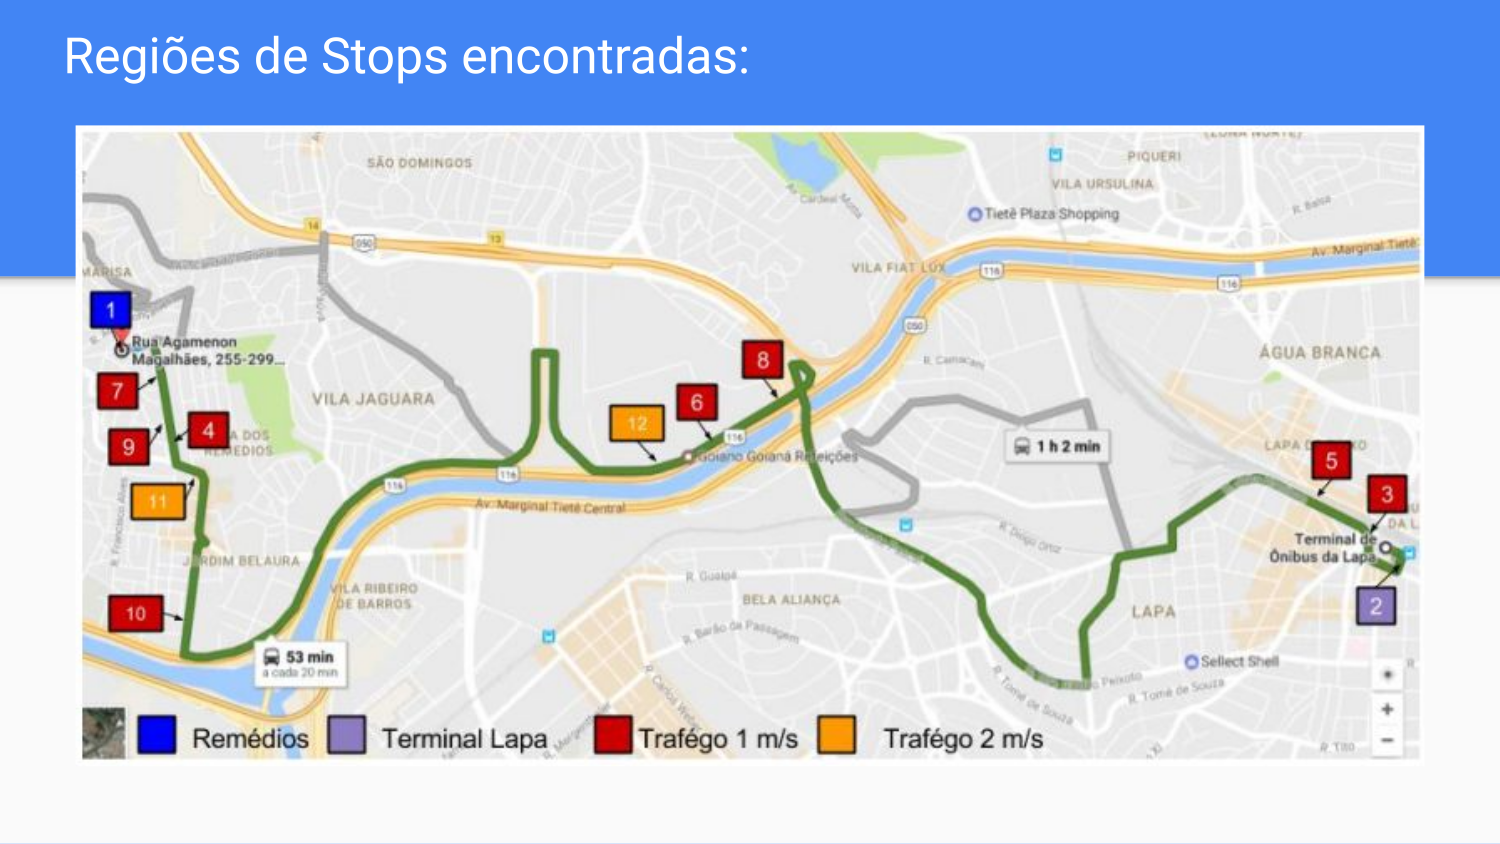
\includegraphics[width=0.9\linewidth]{slide-18.png}
    \caption{Spatial distribution of detected stops. Red markers:
    regions with $v_{\max}=1$~m/s; orange markers: regions with
    $v_{\max}=2$~m/s; purple marker: Terminal Lapa (id 2); blue: Avenida
    dos Remédios endpoint.}
    \label{fig:stops_map}
\end{figure}

\subsection{Qualitative validation}

Each recovered region was cross-checked against street-level imagery.
Figure~\ref{fig:stop3} shows \emph{stop id 3}, Praça Miguel Dell'Erba,
which lies under a viaduct and is regulated by a traffic signal: both
features are consistent with the recurring low-speed behavior captured
by the algorithm. Similar validations for the remaining regions
confirmed either a signalized intersection, a viaduct on-ramp, or a
persistently heavy-traffic stretch of the Marginal Tietê.

\begin{figure}[t]
    \centering
    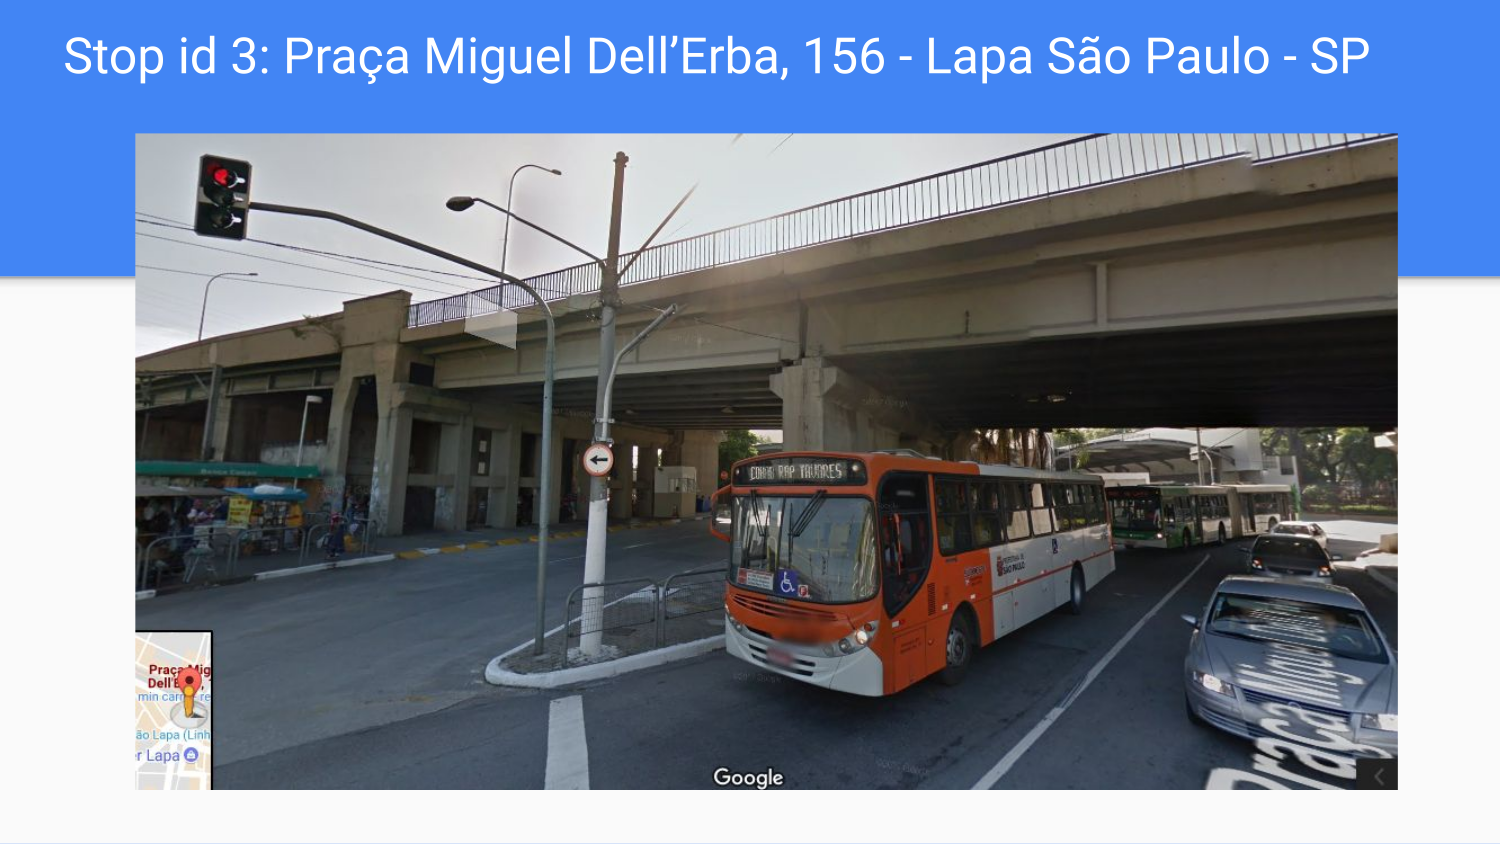
\includegraphics[width=0.75\linewidth]{slide-19.png}
    \caption{Street-level view of \emph{stop id 3}: Praça Miguel
    Dell'Erba, Lapa. The bus is stopped at a red light under a viaduct,
    in a region of high vehicle density — consistent with the
    low-speed signature recovered by CB-SMoT.}
    \label{fig:stop3}
\end{figure}

\section{Discussion}
\label{sec:discussion}

\paragraph{Bus stops versus congestion.}
Of the twelve regions in Table~\ref{tab:stops}, only the terminal
(\emph{id 2}) is explained by scheduled boarding. The remaining eleven
regions all coincide with either signalized intersections, viaducts,
or heavy-traffic corridors. This suggests that, on line 8003-10,
passenger-boarding dwell times do \emph{not} dominate the low-speed
signature of the bus trajectories: the algorithm is effectively
reporting traffic conditions rather than operational stops.

\paragraph{What the algorithm sees.}
Equation~\eqref{eq:stoprule} treats every low-speed event as equivalent;
separating congestion from bus stops and red-light waits ultimately
requires either intersection with external geometries (stop registers,
intersection databases) or a recurrence criterion across days. The
present work automates segment recovery and recurrent-region clustering,
but still performs the address labeling and street-imagery validation
manually, which scales poorly; automating that semantic enrichment is
the natural next step.

\paragraph{Limitations of the Olho Vivo feed.}
Positions are published approximately every 15--20~s, so sub-minute
dynamics (e.g.\ stop-and-go oscillations) are aliased. The feed also
exposes only active vehicles, so buses switched off mid-trip generate
gaps that the $\tau_{\text{gap}}$ cap correctly terminates as
non-stops.

\section{Conclusion}
\label{sec:conclusion}

We applied CB-SMoT to Olho Vivo data on São Paulo bus line 8003-10.
Over a dataset of $2{,}580$ GPS fixes, the algorithm identified twelve
recurring low-speed regions. Manual inspection of street-level imagery
confirmed that the recovered regions correspond to viaducts, signalized
intersections, and heavy-traffic stretches of the Marginal Tietê;
passenger-boarding stops did not emerge as significant contributors on
this route. The pipeline can be reused for continuous monitoring and
analysis over configurable time windows.

Future work includes (i) automating the semantic enrichment step by
intersecting detected segments with SPTrans stop and terminal
geometries and with an intersection database, (ii) aggregating
recurrent stop regions across days to identify stable congestion
hotspots, and (iii) scaling the study from a single line to the full
set of routes exposed by Olho Vivo.

\section*{Code availability}
The implementation is available at
\url{https://github.com/mfilipelino/CB-SMoT}.

\begin{thebibliography}{9}

\bibitem{palma2008}
A.~T.~Palma, V.~Bogorny, B.~Kuijpers, L.~O.~Alvares,
\emph{A Clustering-based Approach for Discovering Interesting Places in
Trajectories}, in Proc.\ ACM Symposium on Applied Computing (SAC), 2008.

\bibitem{alvares2007}
L.~O.~Alvares, V.~Bogorny, B.~Kuijpers, J.~A.~F.~de Macedo,
B.~Moelans, A.~Vaisman,
\emph{A Model for Enriching Trajectories with Semantic Geographical
Information}, in Proc.\ ACM International Symposium on Advances in
Geographic Information Systems (GIS), 2007.

\bibitem{bogorny}
V.~Bogorny, \emph{Trajectory Data Mining: Concepts and Applications}.
Lecture notes / tutorial material, cited in the underlying study.

\bibitem{giannotti}
F.~Giannotti, D.~Pedreschi (eds.), \emph{Mobility, Data Mining and
Privacy --- Geographic Knowledge Discovery}, Springer, 2008.

\end{thebibliography}

\end{document}
